\documentclass[10pt,a4paper]{article}
\usepackage[UTF8,fontset = windows]{ctex}
\setCJKmainfont[BoldFont=黑体,ItalicFont=楷体]{华文中宋}
\usepackage{amssymb,amsmath,amsfonts,amsthm,mathrsfs,dsfont,graphicx}
\usepackage{ifthen,indentfirst,enumerate,color,titletoc}
\usepackage{tikz}
\usepackage{makecell}
\usepackage{longtable}
%\usepackage{mathptmx}

\usetikzlibrary{arrows,calc,intersections,patterns}
\usepackage[bf,small,indentafter,pagestyles]{titlesec}
\usepackage[top=1in, bottom=1in,left=0.8in,right=0.8in]{geometry}
\renewcommand{\baselinestretch}{1.65}
\newtheorem{defi}{定义~}
\newtheorem{eg}{例~}
\newtheorem{ex}{~}
\newtheorem{rem}{注~}
\newtheorem{thm}{定理~}
\newtheorem{coro}{推论~}
\newtheorem{axiom}{公理~}
\newtheorem{prop}{性质~}
\newcommand{\blank}[1]{\underline{\hbox to #1pt{}}}
\newcommand{\bracket}[1]{(\hbox to #1pt{})}
\newcommand{\onech}[4]{\par\begin{tabular}{p{.9\textwidth}}
A.~#1\\
B.~#2\\
C.~#3\\
D.~#4
\end{tabular}}
\newcommand{\twoch}[4]{\par\begin{tabular}{p{.46\textwidth}p{.46\textwidth}}
A.~#1& B.~#2\\
C.~#3& D.~#4
\end{tabular}}
\newcommand{\vartwoch}[4]{\par\begin{tabular}{p{.46\textwidth}p{.46\textwidth}}
(1)~#1& (2)~#2\\
(3)~#3& (4)~#4
\end{tabular}}
\newcommand{\fourch}[4]{\par\begin{tabular}{p{.23\textwidth}p{.23\textwidth}p{.23\textwidth}p{.23\textwidth}}
A.~#1 &B.~#2& C.~#3& D.~#4
\end{tabular}}
\newcommand{\varfourch}[4]{\par\begin{tabular}{p{.23\textwidth}p{.23\textwidth}p{.23\textwidth}p{.23\textwidth}}
(1)~#1 &(2)~#2& (3)~#3& (4)~#4
\end{tabular}}
\begin{document}
\begin{enumerate}[1.]

\item 求函数$y=\dfrac{3x-1}{x+1}$的值域.
\item 求函数$y=\dfrac{4x+3}{2x-1}$的值域.
\item 求函数$y=\dfrac{x^2-1}{x^2+2}$的值域.
\item 求函数$y=\dfrac{x^2-x+1}{2x^2-2x+3}$的值域.
\item 求函数$y=\dfrac{x^2+4x+3}{x^2+x-6}$的值域.
\item 若实数$x,y$满足$x^2+4y^2=4x$, 求$S=x^2+y^2$的值域.
\item 已知函数$y=f(x)=x^2+ax+3$在区间$x\in [-1,1]$上的最小值为$-3$, 求实数$a$的值.
\item 求函数$y=3x^2-12x+18\sqrt {4x-x^2}-23$的值域.
\item 求函数$y=|x-2|-|x+1|$的值域.
\item 若$f(x-1)=2x^2+1$, 求$f(x)$.
\item 已知定义域为$\mathbf{R}$的函数$f(x)$满足:
\textcircled{1} $f(x+y)=f(x)\cdot f(y)$对任何实数$x,y$都成立;
\textcircled{2} 存在实数$x_1,x_2$, 使$f(x_1)\ne f(x_2)$.
求证:\\
(1) $f(0)=1$;\\
(2) $f(x)>0$.
\item 设映射$f:X\to Y$, 其中$X,Y$是非空集合, 则下列语句中正确的是\bracket{20}.
\twoch{$Y$中每一个元素必有原像}{$Y$中的各元素只能有一个原像}{$X$中的不同元素在$Y$中的像也不同}{$Y$中至少存在一个元素, 它有原像}
\item 集合$M=\{a,b,c\}$与$P=\{x,y,z\}$之间建立起四种对应关系(如图), 则下列结论中正确的是\bracket{20}.
\begin{center}
    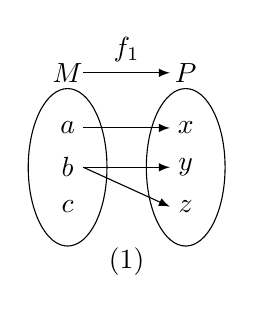
\begin{tikzpicture}[>=latex]
        \draw (0,0) ellipse (0.5 and 1);
        \draw (0,0.5) node {$a$} (0,0) node {$b$} (0,-0.5) node {$c$};
        \draw (1.5,0) ellipse (0.5 and 1);
        \draw (1.5,0.5) node {$x$} (1.5,0) node {$y$} (1.5,-0.5) node {$z$};
        \draw [->] (0.2,0.5) -- (1.3,0.5);
        \draw [->] (0.2,0) -- (1.3,0);
        \draw [->] (0.2,0) -- (1.3,-0.5);
        \draw [->] (0.2,1.2) -- (1.3,1.2);
        \draw (0,1.2) node {$M$} (1.5,1.2) node{$P$};
        \draw (0.75,1.5) node {$f_1$} (0.75,-1.2) node {(1)};
    \end{tikzpicture}
    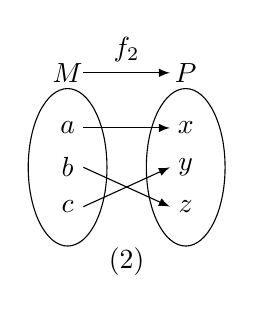
\begin{tikzpicture}[>=latex]
      \draw (0,0) ellipse (0.5 and 1);
      \draw (0,0.5) node {$a$} (0,0) node {$b$} (0,-0.5) node {$c$};
      \draw (1.5,0) ellipse (0.5 and 1);
      \draw (1.5,0.5) node {$x$} (1.5,0) node {$y$} (1.5,-0.5) node {$z$};
      \draw [->] (0.2,0.5) -- (1.3,0.5);
      \draw [->] (0.2,0) -- (1.3,-0.5);
      \draw [->] (0.2,-0.5) -- (1.3,0);
      \draw [->] (0.2,1.2) -- (1.3,1.2);
      \draw (0,1.2) node {$M$} (1.5,1.2) node{$P$};
      \draw (0.75,1.5) node {$f_2$} (0.75,-1.2) node {(2)};
  \end{tikzpicture}
  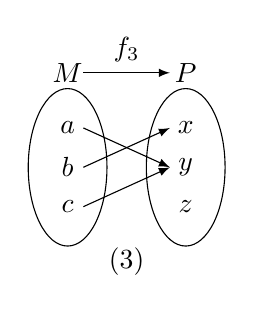
\begin{tikzpicture}[>=latex]
    \draw (0,0) ellipse (0.5 and 1);
    \draw (0,0.5) node {$a$} (0,0) node {$b$} (0,-0.5) node {$c$};
    \draw (1.5,0) ellipse (0.5 and 1);
    \draw (1.5,0.5) node {$x$} (1.5,0) node {$y$} (1.5,-0.5) node {$z$};
    \draw [->] (0.2,0.5) -- (1.3,0);
    \draw [->] (0.2,0) -- (1.3,0.5);
    \draw [->] (0.2,-0.5) -- (1.3,0);
    \draw [->] (0.2,1.2) -- (1.3,1.2);
    \draw (0,1.2) node {$M$} (1.5,1.2) node{$P$};
    \draw (0.75,1.5) node {$f_3$} (0.75,-1.2) node {(3)};
\end{tikzpicture}
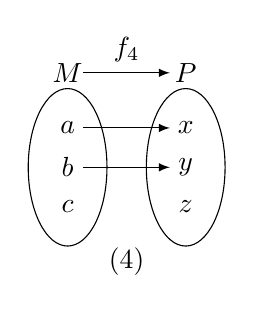
\begin{tikzpicture}[>=latex]
  \draw (0,0) ellipse (0.5 and 1);
  \draw (0,0.5) node {$a$} (0,0) node {$b$} (0,-0.5) node {$c$};
  \draw (1.5,0) ellipse (0.5 and 1);
  \draw (1.5,0.5) node {$x$} (1.5,0) node {$y$} (1.5,-0.5) node {$z$};
  \draw [->] (0.2,0.5) -- (1.3,0.5);
  \draw [->] (0.2,0) -- (1.3,0);
  \draw [->] (0.2,1.2) -- (1.3,1.2);
  \draw (0,1.2) node {$M$} (1.5,1.2) node{$P$};
  \draw (0.75,1.5) node {$f_4$} (0.75,-1.2) node {(4)};
\end{tikzpicture}
\end{center}
\twoch{只有$f_2,f_3$是从$M$到$P$的映射}{只有$f_2,f_4$是从$M$到$P$的映射}{只有$f_3,f_4$是从$M$到$P$的映射}{$f_1,f_2,f_3,f_4$都是从$M$到$P$的映射}
\item 设$(x,y)$在映射$f$下的像是$(\dfrac{x+y}2,\dfrac{x-y}2)$, 则在$f$下$(-5,2)$的原像是\bracket{20}.
\fourch{$(-10,4)$}{$(-3,-7)$}{$(-6,-4)$}{$(-\dfrac 32,-\dfrac 72)$}
\item 在给定的映射$f:(x,y)\mapsto (2x+y,xy)$($x,y\in \mathbf{R}$)下, 点$(\dfrac 16,-\dfrac 16)$的原像是\bracket{20}.
\fourch{$(\dfrac 16,-\dfrac 1{36})$}{$(\dfrac 13,-\dfrac 12)$或$(-\dfrac 14,\dfrac 23)$}{$(\dfrac 1{36},-\dfrac 16)$}{$(\dfrac 12,-\dfrac 13)$或$(-\dfrac 23,\dfrac 14)$}
\item 已知集合$M=\{x|0\le x\le 6\}$, $P=\{0\le y\le 3\}$, 则下列对应关系中, 不能作为从$M$到$P$的映射的是\bracket{20}.
\fourch{$f:x\mapsto y=\dfrac 12x$}{$f:x\mapsto y=\dfrac 13x$}{$f:x\mapsto y=x$}{$f:x\mapsto y=\dfrac 16x$}
\item 设$M=\mathbf{R}$, 从$M$到$P$的映射$f:x\mapsto y=\dfrac 1{x^2+1}$, 则像集$P$为\bracket{20}.
\fourch{$\{y|y\in \mathbf{R}\}$}{$\{y|y\in \mathbf{R}\}$}{$\{y|0\le y\le 2\}$}{$\{y|0<y\le 1\}$}
\item 若映射$f:A\to B$的像集是$Y$, 原像的集合是$X$, 则$X$与$A$的关系是\blank{50}, $Y$和$B$的关系是\blank{50}.
\item 若$(x,y)$在映射$f$下的像是$(2x-y,x+2y)$, 则$(-1,2)$在$f$下的原像是\blank{50}.
\item 已知$(a,b)$在映射$f$的像是$(a-b,ab)$, 则$(2,3)$的原像是\blank{50}.
\item 已知$f:x\mapsto y=x^2$是从集合$\mathbf{R}$到集合$M=\{x|x\ge 0\}$的一个映射, 则$M$中的元素$1$在$\mathbf{R}$中的原像是\blank{50}, $M$中的元素$t$($t>0$)在$\mathbf{R}$中的原像是\blank{50}.
\item 从集合$\{a\}$到$\{b,c\}$的不同映射有\blank{50}个.
\item 从集合$\{1,2\}$到$\{5,6\}$的不同映射有\blank{50}个.
\item 已知集合$A=\mathbf{Z}$, $B=\{x|x=2n+1, \ n\in \mathbf{Z}\}$, $C=\mathbf{R}$, 且从$A$到$B$的映射是$x\mapsto 2x-1$, 从$B$到$C$的映射是$x\mapsto \dfrac 1{3x+1}$, 则从$A$到$C$的映射是\blank{50}.
\item $f$是集合$X=\{a,b,c\}$到集合$Y=\{d,e\}$的一个映射, 则满足映射条件的``$f$''共有\bracket{20}.
\fourch{$5$个}{$6$个}{$7$个}{$8$个}
\item 若$f:y=3x+1$是从集合$A=\{1,2,3,k\}$到集合$B=\{4,7,a^4,a^2+3a\}$的一个映射, 求自然数$a,k$的值及集合$A,B$.
\item 函数$f(x)=\dfrac{\sqrt{x^2-5x+6}}{x-2}$的定义域是\bracket{20}.
\fourch{$\{x|2<x<3\}$}{$\{x|x<2x>3\}$}{$\{x|x\le 2x\ge 3\}$}{$\{x|x<2\text{或}x\ge 3\}$}
\item 若函数$f(x)$的定义域是$[-1,1]$, 则函数$f(x+1)$的定义域是\bracket{20}.
\fourch{$[-1,1]$}{$[0,2]$}{$[-2,0]$}{$[0,1]$}
\item 在\textcircled{1} $y=x$与$y=\sqrt {x^2}$; \textcircled{2} $y=\sqrt {x^2}$与$y=(\sqrt x)^2$; \textcircled{3} $y=|x|$与$y=\dfrac{x^2}x$; \textcircled{4} $y=|x|$与$y=\sqrt {x^2}$; \textcircled{5} $y=x^0$与$y=1$这五组函数中, 表示同一函数的组数是\bracket{20}.
\fourch{$0$}{$1$}{$2$}{$3$}
\item 函数$y=-x^2-2x+3(-5\le x\le 0)$的值域是\bracket{20}.
\fourch{$(-\infty ,4]$}{$[3,12]$}{$[-12,4]$}{$[4,12]$}
\item 已知镭经过$100$年后剩下原来质量的$95.76\%$, 若质量为$l$克的镭经过$x$年后的剩余质量为$y$克, 则$y$与$x$之间的解析式是\bracket{20}.
\fourch{$y=(\dfrac{0.9576}{100})^x$}{$y=(0.9576)^{100x}$}{$y=(0.9576)^{\frac x{100}}$}{$y=1-(1-0.9576)^{\frac x{100}}$}
\item 函数$y=x+\dfrac{|x|}x$的图像是\bracket{20}.
\fourch{\begin{tikzpicture}[scale = 0.7,>=latex]
\draw [->] (-2,0) -- (2,0) node [below] {$x$};
\draw [->] (0,-2) -- (0,2) node [left] {$y$};
\draw (0,0) node [below right] {$O$};
\draw (-1,0) node [below] {$-1$} (0,1) node [right] {$1$};
\draw (-2,-1) -- (1,2);
\filldraw [white] (0,1) circle (0.05);
\draw (0,1) circle (0.05);
\end{tikzpicture}}{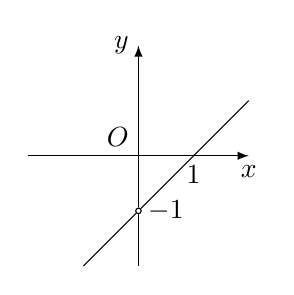
\begin{tikzpicture}[scale = 0.7,>=latex]
\draw [->] (-2,0) -- (2,0) node [below] {$x$};
\draw [->] (0,-2) -- (0,2) node [left] {$y$};
\draw (0,0) node [above left] {$O$};
\draw (1,0) node [below] {$1$} (0,-1) node [right] {$-1$};
\draw (-1,-2) -- (2,1);
\filldraw [white] (0,-1) circle (0.05);
\draw (0,-1) circle (0.05);
\end{tikzpicture}}{\begin{tikzpicture}[scale = 0.7,>=latex]
\draw [->] (-2,0) -- (2,0) node [below] {$x$};
\draw [->] (0,-2) -- (0,2) node [left] {$y$};
\draw (0,0) node [below right] {$O$};
\draw (1,0.1) -- (1,0) node [below] {$1$} (0,-1) node [right] {$-1$} (0,1) node [right] {$1$} (-1,0.1) -- (-1,0) node [below] {$-1$};
\draw (-1,-2) -- (0,-1) (0,1) -- (1,2);
\filldraw [white] (0,-1) circle (0.05);
\draw (0,-1) circle (0.05);
\filldraw [white] (0,1) circle (0.05);
\draw (0,1) circle (0.05);
\end{tikzpicture}}{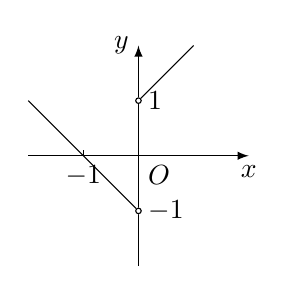
\begin{tikzpicture}[scale = 0.7,>=latex]
\draw [->] (-2,0) -- (2,0) node [below] {$x$};
\draw [->] (0,-2) -- (0,2) node [left] {$y$};
\draw (0,0) node [below right] {$O$};
\draw (0,-1) node [right] {$-1$} (0,1) node [right] {$1$} (-1,0.1) -- (-1,0) node [below] {$-1$};
\draw (-2,1) -- (0,-1) (0,1) -- (1,2);
\filldraw [white] (0,-1) circle (0.05);
\draw (0,-1) circle (0.05);
\filldraw [white] (0,1) circle (0.05);
\draw (0,1) circle (0.05);
\end{tikzpicture}}
\item 函数$y=\sqrt {1-x^2}+\sqrt {x+1}$的定义域为\blank{50}.
\item 函数$y=\dfrac 1{\sqrt {2x^2+3}}$的定义域为\blank{50}.
\item 函数$y=\dfrac{x+5}{3x^2-2x-1}$的定义域为\blank{50}.
\item 函数$y=\sqrt {6x-x^2-9}$的定义域为\blank{50}.
\item 函数$y=\sqrt {4-x^2}+\dfrac 1{|x|-1}$的定义域为\blank{50}.
\item 函数$y=\dfrac{x^3-1}{x+|x|}$的定义域为\blank{50}.
\item 函数$y=\dfrac 1{|x|-x^2}$的定义域为\blank{50}.
\item 函数$y=\sqrt {1-(\dfrac{x-1}{x+1})^2}$的定义域为\blank{50}.
\item 函数$y=\dfrac{\sqrt {x^2-2x-15}}{|x+3|-8}$的定义域为\blank{50}.
\item 函数$y=1-\dfrac 1{x+2}$的值域为\blank{50}.
\item 函数$y=\dfrac 3{2x}$的值域为\blank{50}.
\item 函数$y=\dfrac{x+3}{x-3}$的值域为\blank{50}.
\item 函数$y=\dfrac{5x+3}{x-3}$的值域为\blank{50}.
\item 函数$y=4+\sqrt {2x+1}$的值域为\blank{50}.
\item 函数$y=\sqrt {x-\dfrac 12x^2}$的值域为\blank{50}.
\item 函数$y=\sqrt {-x^2+x+2}$的值域为\blank{50}.
\item 函数$y=\dfrac{2x^2+2x+3}{x^2+x+1}$的值域为\blank{50}.
\item 若函数$f(x)$满足$f(2x)=(1-\sqrt 2x)(1+\sqrt 2x)$, 则$f(x)=$\blank{50}.
\item 若函数$f(x)$满足$f(\sqrt x+1)=x+2\sqrt x$, 则当$x\ge 1$时, $f(x)=$\blank{50}.
\item 若函数$f(x)$满足$f(\dfrac 1x)=\dfrac x{1-x^2}$, 则当$x\ne 0$时, $f(x)=$\blank{50}.
\item 若函数$f(x)=2x+1$, $g(x)=x^2+2$, 满足$f(g(x))=g(f(x))$, 则$x=$\blank{50}.
\item 若函数$f(x)$满足$f(x+1)=2x^2+1$, 则$f(x-1)=$\blank{50}.
\item 若一次函数$f(x)$满足$f(f(x))=1+2x$, 则$f(x)=$\blank{50}.
\item 若$f(x^2-x)=x^4-2x^3+x^2+1$, 则当$x\ge -\dfrac 14$时, $f(f(x))=$\blank{50}.
\item 函数$f(x)=\dfrac x{\sqrt {1+x^2}}$, 则$f(f(x))=$\blank{50}, $f(f(f(x)))=$\blank{50}.
\item 若$-b<a<0$, 且函数$d(x)$的定义域是$[a,b]$, 则函数$F(x)=f(x)+f(-x)$的定义域是\bracket{20}.
\fourch{$[a,b]$}{$[-b,-a]$}{$[-b,b]$}{$[a,-a]$}
\item 若$f(x)$的定义域是$[ 0,1 ]$, 且$f(x+m)+f(x-m)$的定义域是$\varnothing$, 则正数$m$的取值范围是\bracket{20}.
\fourch{$0<m<1$}{$0<m\le \dfrac 12$}{$0<m<\dfrac 12$}{$m>\dfrac 12$}
\item 函数$y=\dfrac{x^2-1}{x^2+1}$的值域是\bracket{20}.
\fourch{$(-1,1)$}{$[-1,1]$}{$[-1,1)$}{$(-1,1]$}
\item 若$2x^2-3x\le 0$, 则函数$f(x)=x^2+x+1$\bracket{20}.
\twoch{有最小值$\dfrac 34$, 但无最大值}{有最小值$\dfrac 34$, 有最大值1}{有最小值1有最大值$\dfrac{19}4$}{既无最小值, 也无最大值}
\item 函数$f(x)=|1-x|-|x-3|(x\in \mathbf{R})$的值域是\bracket{20}.
\fourch{$[-2,2]$}{$[-1,3]$}{$[-3,1]$}{$[0,4]$}
\item 若函数$f(x)$的定义域是$[0,1]$, 分别求函数$f(1-2x)$和$f(x+a)$($a>0$)的定义域.
\item 若函数$f(x+1)$的定义域是$[-2,3)$, 求函数$f(\dfrac 1x+2)$的定义域.
\item 求函数$y=\dfrac{2x}{x^2+x+1}$的值域.
\item 求函数$y=\dfrac{x^2+x-1}{x^2+x+1}$的值域.
\item 求函数$y=\dfrac{x^2-1}{x^2-5x+4}$的值域.
\item 若实数$x,y$满足$3x^2+2y^2=6x$, 分别求$x$与$x^2+y^2$的取值范围.
\item 若实数$x,y$满足$x^2+y^2=2x$, 求$x^2-y^2$的取值范围.
\item 求函数$y=3x-2+\sqrt {3-2x}$的值域.
\item 求函数$y=2x+\sqrt {2x-1}$的值域.
\item 求函数$y=(x-1)(x-2)(x-3)(x-4)+15$的值域.
\item 已知函数$f(x)=x^2-2x+3$在$[0,m]$上有最大值$3$, 最小值$2$, 求正数$m$的取值范围.
\item 已知函数$y=x^2+mx-1$在区间$[0,3]$上有最小值$-2$, 求实数$m$的值.
\item 当$x\ge 0$时, 求函数$f(x)=x^2+2ax$的最小值.
\item 已知函数$f(x)=\dfrac{ax}{2x+3}$($x\ne -\dfrac 32$)满足$f(f(x))=x$, 求实数$a$的值.
\item 已知$f(x)$是二次函数, 且满足$f(2x)+f(3x+1)=13x^2+6x-1$, 求$f(x)$的表达式.
\item 已知函数$f(x)$的定义域是一切非零实数, 且满足$3f(x)+2f(\dfrac 1x)=4x$, 求, $f(x)$的表达式.
\item 作出函数$y=1+\dfrac{|x|}x$的图像.
\item 作出函数$y=x-|1-x|$的图像.
\item 作出函数$y=|x^2-4x+3|$的图像.
\item 作出函数$y=\dfrac{x^3+x}{|x|}$的图像.
\item 作出函数$y=\dfrac{(x+\dfrac 12)}{|x|-x}^0$的图像.
\item 已知$f(x)=-x^2+2x+3$, 画出函数$y=\dfrac 12[f(x)+|f(x)|]$的图像.
\item 已知$f(x)=|x|$, $x\in [-1,1]$, 作出函数$y=f(x+1)+1$的图像.
\item 将进货单价为$40$元的商品按每件$50$元出售时, 每月能卖出$500$个, 已知这批商品在销售单价的基础上每涨价$1$元, 其月销售数就减少$10$个, 为了每月赚取最大利润, 销售单价应定为多少?
\item 飞机飞行$1$小时的耗费由两部分组成: 固定部分$4900$元, 变动部分$P$与飞机飞行速度$v$(千米/时)的函数关系是$P=0.01v^2$. 已知甲、乙两地相距为一常数$a$(千米), 试写出飞机从甲地飞到乙地的总耗费$y$与飞机速度$v$的函数关系式, 并写出耗费最小时飞机的飞行速度.
\item 求证: 函数$f(x)=x^3$在$x\in \mathbf{R}$上是增函数.
\item 已知奇函数$y=f(x)$在$x<0$时是减函数, 求证: $y=f(x)$在$x>0$时也是减函数.
\item 已知$f(x)$是奇函数, 且当$x>0$时$f(x)=x(1-x)$, 求$f(x)$在$x<0$时的表达式.
\item 已知函数$y=f(x)$满足$f(x)=f(4-x)$($x\in \mathbf{R}$), 且$f(x)$在$x>2$时为增函数, 记$a=f(\dfrac 35)$, $b=f(\dfrac 65)$, $c=f(4)$, 则$a,b,c$之间的大小关系是\bracket{20}.
\fourch{$c>a>b$}{$c>b>a$}{$b>a>c$}{$a>c>d$}
\item 画出函数$y=x^2-2|x|-1$的图像.
\item 求函数$y=\dfrac{x-2}{2x+1}$的值域.
\item 已知函数$f(x)=(x-1)^2$($x\le 1$), 又$f(x)$和$\varphi (x)$的图像关于直线$y=x$对称, 求$\varphi (x)$的表达式.
\item 求实数$m$的范围, 使关于$x$的方程$x^2+2(m-1)x+2m+6=0$:\\
(1) 有两个实数根, 且一个比$2$大, 另一个比$2$小;\\
(2) 有两个实数根, 且都比$1$大;\\
(3) 有两个实数根$\alpha ,\beta$, 且满足$0<\alpha <1<\beta <4$;\\
(4) 至少有一个正根.
\item 就参数$m$讨论方程$x^2-2|x|-m=0$的解的情况.
\item 下列记数中, 符合科学记数法的是\bracket{20}.
\fourch{$35.6\times 10^{-25}$}{$0.356\times 10^{-23}$}{$3.56\times 10^{-24}$}{$356\times 10^{-26}$}
\item 计算$3^{-1}\times 2^{-2}\div 4^{-2}$的结果是\bracket{20}.
\fourch{$\dfrac 1{192}$}{$\dfrac 43$}{$\dfrac 1{12}$}{$-\dfrac 43$}
\item 下列各式中, 正确的是\bracket{20}.
\fourch{$(-1)^0=-1$}{$(-1)^{-1}=1$}{$3a^{-2}=\dfrac 1{3a^2}$}{$(-x)^5\div (-x)^3=x^2$}
\item 下列各式中, 计算正确的是\bracket{20}.
\twoch{$(-0.125)\div (-0.5)^{-3}=1$}{$10^{-4}(\sqrt 5)^0=-10000$}{$(\dfrac 13)^0\div 3^{-1}=3$}{$(\sqrt 3-\sqrt 2)^0-(\sqrt 3)^2-(-\sqrt 2)^2=1-3+2=0$}
\item 化简$\dfrac 13x\sqrt {9x}-x^2\sqrt {\dfrac 1x}$的结果是\bracket{20}.
\fourch{$\sqrt x$}{$x(1-x^2)\sqrt x$}{$x^2(1-x\sqrt x)$}{0}
\item 化简$\dfrac{a^{-2}-b^{-2}}{a^2-b^2}$的结果是\bracket{20}.
\fourch{-1}{$-\dfrac 1{a^2b^2}$}{$a^{-1}+b^{-1}$}{$\dfrac 1{a^2b^2}$}
\item 已知$x=1-2^s$, $y=1-2^{-s}$, 则$y$等于\bracket{20}.
\fourch{$\dfrac{x-1}x$}{$\dfrac{2-x}{1-x}$}{$\dfrac x{x-1}$}{$\dfrac{x-2}{x-1}$}
\item 计算$\sqrt {(3-\pi)^2}$的结果是\bracket{20}.
\fourch{$3-\pi$}{$\pi -3$}{$\pi +3$}{$-\pi -3$}
\item 若$(\sqrt [n]{-3})^n$有意义, 则$n$一定是\bracket{20}.
\fourch{正偶数}{自然数}{正奇数}{整数}
\item 已知$n\in \mathbf{N}$, 在\textcircled{1} $\sqrt [4]{(-4)^{2n}}$; \textcircled{2} $\sqrt [4]{(-4)^{2n+1}}$; \textcircled{3} $\sqrt [5]{-x^2}$; \textcircled{4} $\sqrt [5]{-x^2}$这四个式子中, 有意义的\bracket{20}.
\fourch{是\textcircled{1}\textcircled{2}\textcircled{3}\textcircled{4} }{只有\textcircled{3}\textcircled{4}}{只有\textcircled{1}\textcircled{3}\textcircled{4}}{只有\textcircled{4}}
\item 若$\sqrt [4]{4a^2-4a+1}=\sqrt [3]{1-2a}$, 则实数$a$的取值范围是\bracket{20}.
\fourch{$a<2$}{$a=\dfrac 12$或0}{$a>\dfrac 12$}{$R$}
\item 在\textcircled{1} $0^{-1}$; \textcircled{2} $0^{-\frac 12}$; \textcircled{3} $0^0$; \textcircled{4} $0^{0.2}$这四个式子中, 有意义的个数是\bracket{20}.
\fourch{$0$}{$1$}{$2$}{$3$}
\item 下列各式中正确的是\bracket{20}.
\fourch{$-4^0=1$}{$(5^{-\frac 12})^2=5$}{$(-3^{m-n})^2=9^{m-n}$}{$(-2)^{-1}=\dfrac 12$}
\item 计算$[ (-3)^2 ]^{\frac 12}-(-10)^0$的值等于\bracket{20}.
\fourch{$-2$}{$2$}{$-4$}{$4$}
\item 下列计算中正确的是\bracket{20}.
\fourch{$a^{\frac 83}\cdot a^{\frac 38}=a$}{$a^{\frac 83}\cdot a^{-\frac 83}=0$}{$a^{\frac 83}\div a^{\frac 13}=a^8$}{$a^{\frac 12}\div a^{\frac 13}=a^{\frac 16}$}
\item 下列计算中正确的是\bracket{20}.
\fourch{$a^{\frac 34}\cdot a^{\frac 43}=a$}{$a^{\frac 34}\div a^{\frac 34}=a$}{$a^{-4}\div a^4=0$}{$(a^{\frac 34})^{\frac 43}=a$}
\item 化简$(a^{\frac 23}b^{\frac 12})(-3a^{\frac 12}b^{\frac 13})\div (\frac 13a^{\frac 16}b^{\frac 56})$的结果是\bracket{20}.
\fourch{$6a$}{$-a$}{$-9a$}{$9a$}
\item 将$\sqrt [3]{-2\sqrt 2}$化成不含根号的式子是\bracket{20}.
\fourch{$-2^{\frac 12}$}{$-2^{-\frac 12}$}{$-2^{\frac 13}$}{$-2^{\frac 23}$}
\item 将$(a^{\frac 1n}+b^{\frac 1n})^{\frac 13}$表示成根式的形式是\bracket{20}.
\fourch{$\sqrt [3]{a^{\frac 1n}+b^{\frac 1n}}$}{$(\sqrt[n]a+\sqrt[n]b)^{\frac 13}$}{$\sqrt [3]{\sqrt[n]a+\sqrt[n]b}$}{$(\sqrt[n]a+\sqrt[n]b)^3$}
\item 计算: $\sqrt {12}-\sqrt 3\div (2+\sqrt 3)=$\blank{50}.
\item 计算: $(\sqrt {12}-\sqrt {\dfrac 12}-2\sqrt {\dfrac 13})-(\sqrt {\dfrac 18}-\sqrt {18})=$\blank{50}.
\item 计算: $(\sqrt 3+2)^{1997}	\times (\sqrt 3-2)^{1988}=$\blank{50}.
\item 计算: $\dfrac{2\sqrt {10}-5}{4-\sqrt 10}=$\blank{50}.
\item 计算: $4\sqrt {\dfrac 25}-\sqrt {1000}+2\sqrt {10}=$\blank{50}.
\item 计算: $\dfrac 1{(2+\sqrt 3)^2}+\dfrac 1{(2-\sqrt 3)^2}=$\blank{50}.
\item 计算: $\dfrac 1{1+\sqrt 2+\sqrt 3}+\dfrac 1{1-\sqrt 2+\sqrt 3}=$\blank{50}.
\item 将下式改写成不含分数指数幂的根式形式(要求分母不含有根式形式): $3x^{-\frac 32}=$\blank{50}.
\item 将下式改写成不含分数指数幂的根式形式(要求分母不含有根式形式): $a^{\frac 12}\cdot b^{-\frac 12}=$\blank{50}.
\item 将下式改写成不含分数指数幂的根式形式(要求分母不含有根式形式): $(a+b)^{\frac 12}\cdot (a-b)^{-\frac 43}=$\blank{50}.
\item 将根式改写成分数指数幂的形式: $\sqrt [4]{a^3}=$\blank{50}.
\item 将根式改写成分数指数幂的形式: $\sqrt [5]{b^8}=$\blank{50}.
\item 将根式改写成分数指数幂的形式: $\sqrt [4]{x^2+y^2}=$\blank{50}.
\item 将根式改写成分数指数幂的形式: $\dfrac{\sqrt x}{\sqrt [3]{y^4}}=$\blank{50}.
\item 将根式改写成分数指数幂的形式: $\sqrt {2\sqrt 2}=$\blank{50}.
\item 将根式改写成分数指数幂的形式: $-\dfrac 1{\sqrt {27x}}=$\blank{50}.
\item 将根式改写成分数指数幂的形式: $\sqrt {\dfrac 4{3ab^3}}=$\blank{50}.
\item 已知$m<n$, 将根式改写成分数指数幂的形式: $2\sqrt [6]{(m-n)^{-2}}=$\blank{50}.
\item 判断命题: $2^{\frac 32}\cdot 2^{\frac 23}=2$是否正确, \blank{50}.
\item 判断命题: $(\dfrac 18)^{-\frac 12}=-2\sqrt 2$是否正确, \blank{50}.
\item 判断命题: 若$a\in \mathbf{R}$, 则$(a-1)^0=1$是否正确, \blank{50}.
\item 判断命题: $a^x+a^y=a^{x+y}$是否正确, \blank{50}.
\item 判断命题: $\sqrt [3]{-5}=\sqrt [6]{(-5)^2}=\sqrt [6]{25}$是否正确, \blank{50}.
\item 计算: $(\dfrac{81}{625})^{-\frac 34}=$\blank{50}.
\item 计算: $(0.064)^{-\frac 13}=$\blank{50}.
\item 计算: $(2\sqrt 2)^{-\frac 13}=$\blank{50}.
\item 计算: $[ (-3)^2 ]^{\frac 32}=$\blank{50}.
\item 计算: $(-0.027)^{-\frac 23}=$\blank{50}.
\item 计算: $(-0.001)^{-\frac 43}=$\blank{50}.
\item 计算: $5^{\frac 45}\times 125	\times 25^{-0.4}=$\blank{50}.
\item 计算: $(8+2	\times 15^{\frac 12})^{\frac 12}=$\blank{50}.
\item 计算: $(4-12^{\frac 12})^{\frac 12}=$\blank{50}.
\item 计算: $(0.25)^{-0.5}+(\dfrac 1{27})^{-\frac 13}-625^{0.25}=$\blank{50}.
\item 化简: $2x^{-\frac 13}(\dfrac 12x^{\frac 13}-2x^{-\frac 23})-(-3.5)^0=$\blank{50}.
\item 化简: $(x^{\frac 13}+y^{\frac 13})(x^{\frac 23}-x^{\frac 13}y^{\frac 13}+y^{\frac 23})=$\blank{50}.
\item 化简: $(\dfrac{b^3}{2a^2})\div (-\dfrac{4b^3}{a^{-7}})\times (-\dfrac{b^2}a)^3=$\blank{50}.
\item 化简: $(2a^{\frac 14}b^{-\frac 13})(-3a^{-\frac 12}b^{\frac 23})\div (-\frac 14a^{-\frac 14}b^{-\frac 23})=$\blank{50}.
\item 若$a=1.5^{-\frac 12}$, $b=0.5^{-\frac 12}$, $c=1$, 则它们的大小顺序是\bracket{20}.
\fourch{$a<c<b$}{$a<b<c$}{$c<b<a$}{$b<c<a$}
\item 若$a=\dfrac 1{\sqrt 2}$, $b=\dfrac 1{\sqrt[3]2}$, 则$[a^{-\frac 32}b(ab^{-2})^{-\frac 12}(a^{-1})^{-\frac 23}]^3=$\blank{50}.
\item 若$a^{\frac 12}+a^{-\frac 12}=2$, 则:\\
(1) $a+a^{-1}=$\blank{50};\\
(2) $a^2+a^{-2}=$\blank{50};\\
(3) $a^4+a^{-4}=$\blank{50}.
\item 若$10^{\alpha }=2^{-\frac 12}$, $10^{\beta }=\sqrt [3]{32}$, 则$10^{2\alpha -\frac 34\beta }=$\blank{50}.
\item 计算: $(\dfrac 1{125})^{-\frac 13}+(-2)^{-2}+(-2)^0$.
\item 计算: $(2\dfrac 79)^{\frac 12}-(-0.027)^{-\frac 13}-(-\sqrt 3)^{-2}+\pi ^0$.
\item 计算: $5-3\times [ (-3\dfrac 38)^{-\frac 13}+1031\times (0.25-2^{-2}) ]\div 9^0$.
\item 计算: $(0.027)^{\frac 13}-(-\dfrac 16)^{-2}+256^{0.75}-|-3^{-1}|+(-5.555)^0$.
\item 计算: $(2.25)^{0.5}+(-4.3)^0-(3\dfrac 38)^{-\frac 23}+\dfrac{3^{-2}-2^{-2}}{3^{-1}-2^{-1}}$.
\item 计算: $(0.25)^{-2}+(\dfrac 8{27})^{\frac 13}+(\dfrac 18)^{-\frac 23}-(\dfrac 1{16})^{-0.75}$.
\item 计算或化简: $\sqrt [3]{m^{\frac 92}\cdot \sqrt {m^{-3}}}\div \sqrt {\sqrt [3]{m^{-7}}}\cdot \sqrt [3]{m^{13}}(m>0)$.
\item 计算或化简: $(x-y)\div (x^{\frac 12}+y^{\frac 12})-(x+y-2x^{\frac 12}y^{\frac 12})\div (x^{\frac 12}-y^{\frac 12})(x>y>0)$.
\item 计算或化简: $(8y^{-\frac 13}\sqrt {x^{-\frac 13}y\sqrt {x^{\frac 43}}})^{\frac 13}$.
\item 计算或化简: $\dfrac{x+y}{\sqrt x+\sqrt y}+\dfrac{2xy}{x\sqrt y+y\sqrt x}$.
\item 计算或化简: $(5+\sqrt 6+\sqrt {10}+\sqrt {15})\div (\sqrt 2+\sqrt 3+\sqrt 5)$.
\item 计算或化简: $(2+3^\frac 12)^\frac 12\times (2+(2+3^\frac 12)^\frac 12)^\frac 12\times (2+(2+(2+3^\frac 12)^\frac 12)^\frac 12)^\frac 12$.
\item 化简: $\sqrt {x+2\sqrt {x-1}}+\sqrt {x-2\sqrt {x-1}}$.
\item 化简: $(x^{\frac{a+b}{c-a}})^{\frac 1{b-c}}\cdot (x^{\frac{x+a}{b-c}})^{\frac 1{a-b}}\cdot (x^{\frac{b+c}{a-b}})^{\frac 1{c-a}}$.
\item 化简: $\dfrac{a^2-b^2}{a^2+b^2}(\dfrac{a-b}{a+b})^{\frac{p+q}{p-q}}\cdot [(\dfrac{a+b}{a-b})^{\frac{2p}{p-q}}+(\dfrac{a+b}{a-b})^{\frac{2q}{p-q}}]$.
\item 当$a=0.001$时, 求$\dfrac{a^{\frac 43}-8a^{\frac 13}b}{a^{\frac 23}+2\sqrt [3]{ab}+4b^{\frac 23}}\div (1-2\sqrt [3]{\frac ba})$的值.
\item 求证: $\dfrac 1{1+x^{a-b}+x^{a-c}}+\dfrac 1{1+x^{b-c}+x^{b-a}}+\dfrac 1{1+x^{c-a}+x^{c-b}}=1$.
\item 已知幂函数$f(x)$的图像经过点$(2,\dfrac{\sqrt 2}2)$, 则$f(4)$的值等于\bracket{20}.
\fourch{$16$}{$\dfrac 1{16}$}{$\dfrac 12$}{$2$}
\item 下列幂函数中, 定义域为$\{x|x>0\}$的是\bracket{20}.
\fourch{$y=x^{\frac 23}$}{$y=x^{\frac 32}$}{$y=x^{-\frac 23}$}{$y=x^{-\frac 32}$}
\item 幂函数$y=x^n(n\in \mathbf{Z})$的图像一定不经过\bracket{20}.
\fourch{第一象限}{第二象限}{第三象限}{第四象限}
\item 函数$f(x)=x^{\frac 23}$的图像是\bracket{20}.
\fourch{\begin{tikzpicture}[scale = 0.7, >=latex]
\draw [->] (-2,0) -- (2,0) node [below] {$x$};
\draw [->] (0,-2) -- (0,2) node [left] {$y$};
\draw (0,0) node [below left] {$O$};
\draw (1,0.2) -- (1,0) node [below] {$1$};
\draw (0.2,1) -- (0,1) node [left] {$1$};
\draw [domain = 0:4,samples = 400] plot ({\x^(1/2)},{\x^(1/3)});
\end{tikzpicture}}{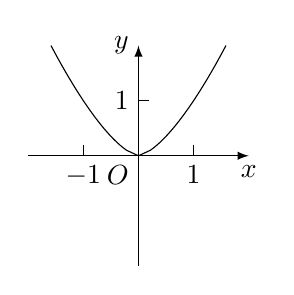
\begin{tikzpicture}[scale = 0.7, >=latex]
\draw [->] (-2,0) -- (2,0) node [below] {$x$};
\draw [->] (0,-2) -- (0,2) node [left] {$y$};
\draw (0,0) node [below left] {$O$};
\draw (1,0.2) -- (1,0) node [below] {$1$};
\draw (0.2,1) -- (0,1) node [left] {$1$};
\draw (-1,0.2) -- (-1,0) node [below] {$-1$};
\draw [domain = 0:4,samples = 400] plot ({\x^(1/3)},{\x^(1/2)});
\draw [domain = 0:4,samples = 400] plot ({-\x^(1/3)},{\x^(1/2)});
\end{tikzpicture}}{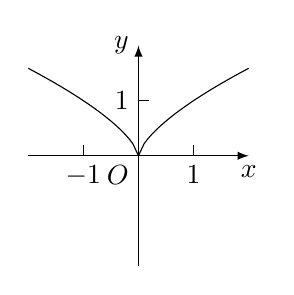
\begin{tikzpicture}[scale = 0.7, >=latex]
\draw [->] (-2,0) -- (2,0) node [below] {$x$};
\draw [->] (0,-2) -- (0,2) node [left] {$y$};
\draw (0,0) node [below left] {$O$};
\draw (1,0.2) -- (1,0) node [below] {$1$};
\draw (0.2,1) -- (0,1) node [left] {$1$};
\draw (-1,0.2) -- (-1,0) node [below] {$-1$};
\draw [domain = 0:4,samples = 400] plot ({\x^(1/2)},{\x^(1/3)});
\draw [domain = 0:4,samples = 400] plot ({-\x^(1/2)},{\x^(1/3)});
\end{tikzpicture}}{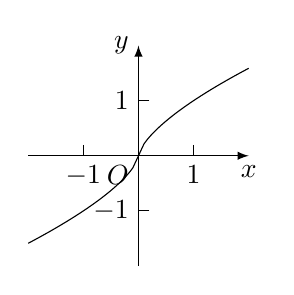
\begin{tikzpicture}[scale = 0.7, >=latex]
\draw [->] (-2,0) -- (2,0) node [below] {$x$};
\draw [->] (0,-2) -- (0,2) node [left] {$y$};
\draw (0,0) node [below left] {$O$};
\draw (1,0.2) -- (1,0) node [below] {$1$};
\draw (0.2,1) -- (0,1) node [left] {$1$};
\draw (-1,0.2) -- (-1,0) node [below] {$-1$};
\draw (0.2,-1) -- (0,-1) node [left] {$-1$};
\draw [domain = 0:4,samples = 400] plot ({\x^(1/2)},{\x^(1/3)});
\draw [domain = 0:4,samples = 400] plot ({-\x^(1/2)},{-\x^(1/3)});
\end{tikzpicture}}
\item 幂函数$y=x^m$和$y=x^n$在第一象限内的图像$C_1$和$C_2$图像所示, 则$m,n$之间的关系是\bracket{20}.
\begin{center}
    \begin{tikzpicture}[>=latex]
        \draw [->] (-1,0) -- (3,0) node [below] {$x$};
        \draw [->] (0,-1) -- (0,3) node [left] {$y$};
        \draw (0,0) node [below left] {$O$};
        \draw (1,0.2) -- (1,0) node [below] {$1$};
        \draw (0.2,1) -- (0,1) node [left] {$1$};
        \draw [domain = 0.5:2, samples = 400] plot (\x,{\x^(-5/4)});
        \draw [domain = 0.5:2, samples = 400] plot ({\x^(-5/4)},\x);
        \draw (0.5,{0.5^(-5/4)}) node [right] {$C_2$} ({0.5^(-5/4)},0.5) node [above] {$C_1$};
    \end{tikzpicture}
\end{center}
\fourch{$n<m<0$}{$m<n<0$}{$n>m>0$}{$m>n>0$}
\item 图中, $C_1,C_2,C_3$为幂函数$y=x^a$在第一象限的图像, 则解析式中的指数$\alpha$依次可以取\bracket{20}.
\begin{center}
    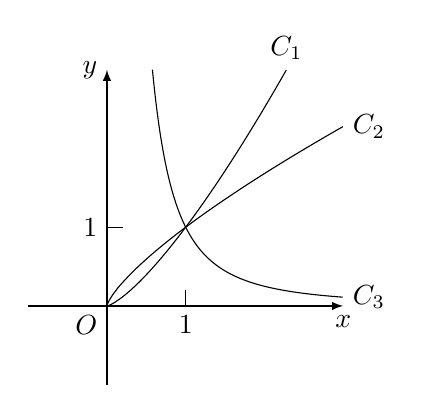
\begin{tikzpicture}[>=latex]
        \draw [->] (-1,0) -- (3,0) node [below] {$x$};
        \draw [->] (0,-1) -- (0,3) node [left] {$y$};
        \draw (0,0) node [below left] {$O$};
        \draw (1,0.2) -- (1,0) node [below] {$1$};
        \draw (0.2,1) -- (0,1) node [left] {$1$};
        \draw [domain = {sqrt(3)/3}:3, samples = 400] plot (\x,{\x^(-2)});
        \draw [domain = 0:3, samples = 400] plot (\x,{\x^(3/4)});
        \draw [domain = 0:{3^(3/4)}, samples = 400] plot (\x,{\x^(4/3)});
        \draw (3,{1/9}) node [right] {$C_3$} (3,{3^(3/4)}) node [right] {$C_2$} ({3^(3/4)},3) node [above] {$C_1$};
    \end{tikzpicture}
\end{center}
\fourch{$\dfrac 43,-2,\dfrac 34$}{$-2,\dfrac 34,\dfrac 43$}{$-2,\dfrac 43,\dfrac 34$}{$\dfrac 34,\dfrac 43,-2$}
\item 函数$y=x^{\frac 56}$的定义域为\blank{50}, 值域为\blank{50}.
\item 函数$y=x^{\frac 35}$的定义域为\blank{50}, 值域为\blank{50}.
\item 函数$y=x^{\frac 85}$的定义域为\blank{50}, 值域为\blank{50}.
\item 函数$y=x^{-\frac 54}$的定义域为\blank{50}, 值域为\blank{50}.
\item 函数$y=x^{-\frac 53}$的定义域为\blank{50}, 值域为\blank{50}.
\item 函数$y=x^{-\frac 23}$的定义域为\blank{50}, 值域为\blank{50}.
\item 函数$y=-2(x+5)^{-\frac 14}$的定义域为\blank{50}, 值域为\blank{50}.
\item 函数$y=5(2x-1)^{\frac 34}$的定义域为\blank{50}, 值域为\blank{50}.
\item 将下列函数图像的标号, 填在相应函数后面的横线上:\\
(1) $y=x^{\frac 23}$:\blank{50}; (2) $y=x^{-2}$:\blank{50}; (3) $y=x^{\frac 12}$:\blank{50};\\
(4) $y=x^{-1}$:\blank{50}; (5) $y=x^{\frac 13}$:\blank{50}; (6)$y=x^{\frac 32}$:\blank{50};\\ (7)$y=x^{\frac 43}$:\blank{50}; (8)$y=x^{-\frac 12}$:\blank{50}; (9)$y=x^{\frac 53}$:\blank{50}.

\item (1)若幂函数$y=x^n$的图像在$0<x<1$时位于直线$y=x$的下方, 则$n$的取值范围是\blank{50}.
(2)若幂函数$y=x^n$的图像在$0<x<1$时位于直线$y=x$的上方, 则$n$的取值范围是\blank{50}.
*(3)函数$f(x)=x^{k^2-2k-3}$($k\in \mathbf{Z}$)的图像如图所示, 则$k=$\blank{50}.
(第76(3)题)
\item 幂函数$y=x^p$与$y=x^q$的图像都通过定点\blank{50}, 它们在第一象限部分关于直线$y=x$对称, 则$p,q$应满足的条件是\blank{50}.
\item 确定实数$a$的取值范围:
(1)$2.4^a>2.5^a.$				(2)$(\dfrac 34)^{-a}>(\dfrac 43)^{-a}.$
(3)$a^{-2}>3^{-2}.$				(4)$0.01^{-3}>a^{-3}.$
\item 将下列各组数从小到大排列:
(1)$2.5^{\frac 23}$, $(-1.4)^{\frac 23}$, $(-3)^{\frac 13}$:\blank{50}.
(2)$4.1^{\frac 25}$, $3.8^{-\frac 23}$, $(-1.9)^{\frac 35}$:\blank{50}.
(3)$0.16^{-\frac 34}$, $0.5^{-\frac 32}$, $6.25^{\frac 38}$:\blank{50}.
\item 已知函数$y=x^{n^2-2n-3}$($n\in \mathbf{Z}$)的图像与两坐标轴都无公共点, 且其图像关于$y$轴对称, 求$n$的值, 并画出相应的函数图像.
(三)函数的单调性
\item 函数$y=\sqrt {x^2+2x-3}$为减函数的区间是\bracket{20}.
\fourch{$(-\infty ,-3 ].$}{$[ -1,+\infty).$}{$(-\infty ,-1 ].$}{$[ 1,+\infty).$}
\item 若函数$y=(2k+1)x+b$在$(-\infty ,+\infty)$上是减函数, 则\bracket{20}.
\fourch{$k>\dfrac 12.$}{$k<\dfrac 12.$}{$k>-\dfrac 12.$}{$k<-\dfrac 12.$}
\item 若函数$f(x)=4x^2-mx+5$在区间$[ -2,+\infty)$上是增函数, 在区间$(-\infty ,-2 ]$上是减函数, 则$f(1)$等于\bracket{20}.
\fourch{$-7.$}{1}{17}{25}
\item 若函数$y=x^2+2(a-2)x+5$在区间$(4,+\infty)$上是增函数, 则实数$a$的取值范围是\bracket{20}.
\fourch{$a\le -2.$}{$a\ge -2.$}{$a\le -6.$}{$a\ge -6.$}
\item 下列函数中, 在区间$(0,2)$上为增函数的是\bracket{20}.
\fourch{$y=-3x+1.$}{$y=\sqrt[3]x.$}{$y=x^2-4x+3.$}{$y=\dfrac 4x.$}
\item 若函数$f(x)$在定义域$R$上为增函数, 且$f(x)<0$, 则下列函数在$R$上为增函数的是\bracket{20}.
\fourch{$y=|f(x)|.$}{$y=\dfrac 1{f(x)}$}{$y=[ f(x) ]^2.$}{$y=[ f(x) ]^3.$}
\item (1)函数$y=\dfrac 1{\sqrt {x^2-4x+5}}$为增函数的区间是\blank{50}, 为减函数的区间是\blank{50}.
(2)函数$y=\dfrac 1{\sqrt {3+2x-x^2}}$为增函数的区间是\blank{50}.
(3)函数$y=|3x-5|$为减函数的区间是\blank{50}.
(4)函数$y=|x^2-2x-3|$为增函数的区间是\blank{50}.
(5)函数$y=\dfrac{1-x}{1+x}$为减函数的区间是\blank{50}.
\item 定义在[1, 3]上的函数$f(x)$为减函数, 求满足不等式$f(1-a)-f(3-a^2)>0$的解集.
\item (1)已知$f(x)=-x^3-x+1$($x\in \mathbf{R}$), 求证$y=f(x)$在定义域上为减函数.
(2)求证: 函数$f(x)=x+\dfrac 1x$在(0, 1)上是减函数, 在$(1,+\infty)$上是增函数.
(3)求证: $f(x)=\sqrt x-\dfrac 1x$在定义域上是增函数.
(4)已知常数$m,n$满足$mn<2$, 求证: 函数$f(x)=\dfrac{mx+1}{2x+n}$在$(-\dfrac n2,+\infty)$上为减函数.
\item 已知$f(x)=x^2+1$, $g(x)=x^4+2x^2+2$, 是否存在实数$\lambda$, 使得$F(x)=g(x)-\lambda f(x)$在$(-\infty ,-1)$上是减函数, 在(-1, 0)上是增函数?
\item 已知函数$f(x)$在区间$(-\infty ,+\infty)$上是增函数, 又实数$a,b$满足$a+b\ge 0$, 求证: $f(a)+f(b)\ge f(-a)+f(-b)$.
\item $f(x)$是定义在$\mathbf{R}^+$的增函数, 且$f(\dfrac xy)=f(x)-f(y)$.
(1)求$f(1)$的值.
(2)若$f(6)=1$, 解不等式$f(x+3)-f(\dfrac 1x)<2$.
(四)函数的奇偶性
\item 若$f(x)=(m-1)x^2+3mx+3$为偶函数, 则$f(x)$在区间(-4, 2)上\bracket{20}.
\fourch{是增函数}{是减函数}{先是增函数后是减函数}{先是减函数后是增函数}
\item 函数$f(x)=\begin{cases}   1-x, & x>0,  \\ 0, & x=0,  \\1+x, & x<0,  \end{cases}$则该函数\bracket{20}.
\twoch{是奇函数, 但不是偶函数}{是偶函数, 但不是奇函数}{既是奇函数, 也是偶函数}{既不是奇函数, 也不是偶函数}
\item 下列函数中既是奇函数, 又在定义域上为增函数的是\bracket{20}.
\fourch{$f(x)=3x+1.$}{$f(x)=\dfrac 1x.$}{$f(x)=1-\dfrac 1x.$}{$f(x)=x^3.$}
\item 若$f(x)$为定义在区间[-6, 6]上的偶函数, 且满足$f(3)>f(1)$, 则恒成立的是\bracket{20}.
\fourch{$f(-1)<f(3).$}{$f(0)<f(6).$}{$f(3)>f(2).$}{$f(2)>f(0).$}
\item 函数$f(x)=\dfrac{\sqrt {1-x^2}}{2-|x+2|}$\bracket{20}.
\twoch{是奇函数, 但不是偶函数}{是偶函数, 但不是奇函数}{既是奇函数, 又是偶函数}{既不是奇函数, 也不是偶函数}
\item 已知$f(x)$是奇函数, 则下列各点中在函数$y=f(x)$的图像上的点的是\bracket{20}.
\fourch{$(a,f(-a)).$}{$(-a,-f(a)).$}{$(\dfrac 1a,-f(\dfrac 1a)).$}{$(-\sin a,-f(-\sin a)).$}
\item (1)若$f(x)$是定义在$R$上的偶函数, 且当$x<0$时, $f(x)=2x-3$, 则当$x>0$时, $f(x)=$\blank{50}.
(2)若奇函数$f(x)$的定义域是$R$, 则$f(0)=$\blank{50}.
\item (1)若奇函数$f(x)$在区间[-3, -1]上是增函数, 且有最大值-2, 则$f(x)$在[1, 3]上是\blank{50}函数(填``增''或``减''), 且最小值等于\blank{50}.
(2)设$f(x)$为定义在$R$上的偶函数, 且$f(x)$在$[ 0,+\infty)$上是增函数, 则$f(-4)$, $f(-2)$, $f(3)$由小到大的排列顺序为\blank{50}.


\end{enumerate}
\end{document}